\documentclass[10pt, compress]{beamer}

\usetheme{metropolis}
\usepackage{appendixnumberbeamer}

\usepackage{tikz-dependency}
\usepackage{tikz}
\usepackage{tikz-qtree}

\usepackage{caption}
\usepackage{booktabs}
\usepackage{tabularx}
\usepackage{multicol}
\usepackage{alltt}
\usepackage[scale=2]{ccicons}

\usepackage{pgfplots}
\usepgfplotslibrary{dateplot}

\usepackage{xspace}
\newcommand{\themename}{\textbf{\textsc{metropolis}}\xspace}

% commands from the paper
\newfontfamily\gtfont[Scale=1.1,Letters=SmallCaps]{Linux Libertine O}
\newcommand{\udtag}[1]{{\ll \textsc{#1}}}
\newcommand{\gtlabel}[1]{{\gtfont #1}}
\newcommand{\udlabel}[1]{{\tt #1}}
\newfontfamily\udfont[Scale=0.9,Letters=SmallCaps]{Linux Libertine O}
\newcommand{\utag}[1]{{\udfont#1}}
\newcommand{\ufeat}[1]{{\udfont#1}}
\newcommand{\tgl}[1]{{\em #1}}
\setmonofont[Scale=MatchLowercase]{DejaVu Sans Mono}

% commands from the paper


\newcommand{\myarrow}[1][-45]{%
  \mathrel{%
    \text{$
     \begin{tikzpicture}[baseline = -0.5ex]
       \node[inner sep=0pt,outer sep=0pt,rotate = #1] (a) at (0,0)  {$\xrightarrow{}$};
    \end{tikzpicture}
    $}%
  }%
}%




\title{Class 07: Semantic roles and PropBank}
\date{}
\begin{document}

\maketitle

\begin{frame}{Introduction}

% Что сделал кто кому ?

The grand quest of NLP: \\
~\\
\begin{center}
\begin{tabular}{cccc}
  Кто ?      &   сделал что ? & кому ? & где ? \\
{\Large Маша} & {\Large продала книгу} & {\Large Даше} & {\Large в метро} \\
 \emph{Maša} & \emph{sold the book} & \emph{to Daša} & \emph{on the metro} \\
\end{tabular}
\end{center}

\begin{itemize}
  \item Что было сделано ?
  \item Кто продал книгу? 
  \item Кому продала Маша книгу ? / Кому Маша продала книгу ?
  \item Где Маша продала книгу ?
\end{itemize}

\end{frame}

\begin{frame}

\begin{itemize}
  \item Question answering 
  \begin{itemize}
    \item Determining if an event corresponds to a question
    \item Event extraction and ontology filling
  \end{itemize}
  \item Machine translation
  \begin{itemize}
     \item Evaluation: Text coherence
     \item Features for argument structure coherence
     \begin{itemize}
       \item Making sure the ``who did what to whom'' is preserved in the output
     \end{itemize}
  \end{itemize}
\end{itemize} 

\end{frame}

\begin{frame}{Syntax/1}
% Isn't this solved by dependency parsing ?

\begin{onlyenv}<1>
\begin{center}
\Tree [.S [.NP Маша ] [.VP [.VP [.VP [.V продала ] [.NP книгу ] ] [.AdvP Даше ] ] [.PP [.Prep в ] [.NP метро ] ] ] ]
\end{center}
\end{onlyenv}
\begin{onlyenv}<2>
\begin{center}
\Tree [.S [.VP [.PP [.Prep В ] [.NP метро ] ] [.VP [.V продала ] [.NP книгу ] ] ] [.NP Маша ] [.AdvP Даше ] ]
\end{center}
\end{onlyenv}

\end{frame}


\begin{frame}{Syntax/2}

Doesn't dependency parsing solve this ? 

\begin{center}

    \begin{dependency}
      \begin{deptext}[column sep=1mm,column 1/.style={anchor=base west}]
			Маша \& продала \& книгу \& Даше \& в \& метро \\  
        \end{deptext}
        \depedge{2}{1}{nsubj}
        \depedge{2}{3}{obj}
        \depedge{2}{4}{obl}
        \depedge{6}{5}{case}
        \depedge{2}{6}{obl}
    \end{dependency}

    \begin{dependency}
      \begin{deptext}[column sep=1mm,column 1/.style={anchor=base west}]
			В \& метро \& продала \& Маша \& книгу \& Даше \\
        \end{deptext}
        \depedge{3}{4}{nsubj}
        \depedge{3}{5}{obj}
        \depedge{3}{6}{obl}
        \depedge{2}{1}{case}
        \depedge{3}{2}{obl}
    \end{dependency}

\end{center}


\end{frame}

\begin{frame}{}

\begin{center}

\begin{columns}

\begin{column}{0.5\textwidth}

\scalebox{0.8}{
    \begin{dependency}
      \begin{deptext}[column sep=1mm,column 1/.style={anchor=base west}]
			Маша \& продала \& книгу \& Даше \& в \& метро \\  
        \end{deptext}
        \depedge{2}{1}{nsubj}
        \depedge{2}{3}{obj}
        \depedge{2}{4}{obl}
        \depedge{6}{5}{case}
        \depedge{2}{6}{obl}
    \end{dependency}
}
\scalebox{0.7}{
    \begin{dependency}
      \begin{deptext}[column sep=1mm,column 1/.style={anchor=base west}]
			Книга \& была \& продана \& Машей \& Даше \& в \& метро \\  
        \end{deptext}
        \depedge{3}{1}{nsubj}
        \depedge{3}{2}{aux}
        \depedge{3}{4}{obl}
        \depedge{3}{5}{obl}
        \depedge{7}{6}{obl}
        \depedge{3}{7}{obl}
    \end{dependency}
}

\end{column}
\begin{column}{0.5\textwidth}
\scalebox{0.8}{
    \begin{dependency}
      \begin{deptext}[column sep=1mm,column 1/.style={anchor=base west}]
			Даша \& купила \& книгу \& у \& Даши \& в \& метро \\  
        \end{deptext}
        \depedge{2}{1}{nsubj}
        \depedge{2}{3}{obj}
        \depedge{2}{5}{obl}
        \depedge{2}{7}{obl}
        \depedge{5}{4}{case}
        \depedge{7}{6}{case}
    \end{dependency}
}


\scalebox{0.8}{
    \begin{dependency}
      \begin{deptext}[column sep=1mm,column 1/.style={anchor=base west}]
			Продажа \& книги \& Машей \& в  \& метро \& \ldots \\
        \end{deptext}
        \depedge{1}{2}{nmod}
        \depedge{1}{3}{nmod}
        \depedge{1}{5}{nmod}
        \depedge{5}{4}{case}
    \end{dependency}
}

\end{column}
\end{columns}

Could these refer to the same event ? 

\begin{onlyenv}<2>
Can you think of more ways of saying the same thing?
\end{onlyenv}

\end{center}

%{\Large Википедия была прочитана Машей в метро.}
%{\Large Прочтение Википедии Машей в метро \ldots}

\end{frame}

\begin{frame}[standout]
  Semantic roles
\end{frame}


\begin{frame}{Shallow representation}

Predicates and arguments/roles. \\

Predicates (like продать, купить) represent an \textbf{event}. \\

Semantic roles (like Agent, Theme) express the abstract role of the arguments of the predicate. \\

% Reader     Agent     Proto-Agent

\begin{center}
\begin{tabular}{cccccc}
              & {\Large Buyer}        &  {\Large Agent} & {\Large Proto-Agent}      &   \\
              & $ {\Large \leftarrow}$ &                 & $ {\Large \rightarrow} $  &  \\
              & \textbf{More specific} &                  &  \textbf{More general}   &
  
\end{tabular}
\end{center}

\end{frame}

\begin{frame}{Deep roles}

Specific for a predicate,

\begin{itemize}
  \item Maša broke the window 
  \item Saša opened the door
\end{itemize}

Subjects of \emph{break} and \emph{open}: {\bf Breaker} and {\bf Opener}

The objects are: {\bf BrokenThing} and {\bf OpenedThing}

Hard to reason with for applications

\end{frame}


\begin{frame}{Thematic roles/1}

But both \textbf{Breaker} and \textbf{Opener} have something in common:
\begin{itemize}
  \item Volitional actors
  \item Often animate
  \item Direct causal responsibility for their events
\end{itemize} 

Thematic roles capture this similarity,
\begin{itemize}
\item \textbf{Breaker} and \textbf{Opener} are both {\sc agents}
\begin{itemize}
  \item Volitional actors with causal responsibility for an event
\end{itemize}
\item \textbf{BrokenThing} and \textbf{OpenedThing} are both {\sc themes}
\begin{itemize}
  \item Inanimate objects affected in some way by an action
\end{itemize}
\end{itemize}

\end{frame}

\begin{frame}{Thematic roles/2}
\begin{flushright}
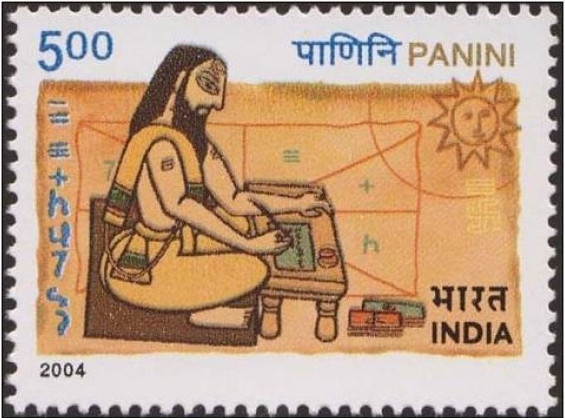
\includegraphics[width=0.3\textwidth]{graphics/panini.jpg}
\end{flushright}
One of the first linguistic models:
\begin{itemize}
  \item Introduced by the grammarian Pāṇini between the 7th and 4th centuries BCE
  \item Called \emph{kāraka} in Sanskrit/Indo-Aryan linguistics
\end{itemize}

Modern formulation by Fillmore (1966):
\begin{itemize}
  \item Influenced by Tesnière (1959)'s dependency syntax
  \item Called first \emph{actants} (following Tesnière) and then later \emph{case}
\end{itemize}

The terminology is confusing.

\end{frame}

\begin{frame}{Thematic roles/3}

\begin{onlyenv}<1>
\begin{center}
\begin{small}
\begin{tabular}{ll}
  \textbf{Role} & \textbf{Definition} \\
 \hline
  {\sc agent}  & The volitional causer of an event \\
               & \ldots \\
  {\sc experiencer} & The experiencer of an event  \\
                    & \ldots \\
  {\sc force} & Non-volitional causer of an event  \\
              & \ldots \\
  {\sc theme} & Participant most directly affected by an event  \\
              & \ldots \\
  {\sc instrument} & An instrument used in an event \\
                 & \ldots \\
  {\sc beneficiary} & The beneficiary of an event \\
                 & \ldots \\
  {\sc source} & Origin of a transfer event \\
              & \ldots \\
  {\sc goal} & The destination of a transfer event \\
               & \ldots \\
 \hline
\end{tabular} 
\end{small}
\end{center}
\end{onlyenv}


\begin{onlyenv}<2>
\begin{center}
\begin{small}
\begin{tabular}{ll}
  \textbf{Role} & \textbf{Definition} \\
 \hline
  {\sc agent}  & The volitional causer of an event \\
               & \textbf{Маша} разбила окно \\
  {\sc experiencer} & The experiencer of an event  \\
                    & \textbf{У Саши} болит голова \\
  {\sc force} & Non-volitional causer of an event  \\
              & \textbf{Ветер} сдувал снег \\ 
  {\sc theme} & Participant most directly affected by an event  \\
              & Маша продала \textbf{книгу} \\
  {\sc instrument} & An instrument used in an event \\
                 & Она написала письмо \textbf{ручкой} \\
  {\sc beneficiary} & The beneficiary of an event \\
                 & Я купил \textbf{тебе} кофе \\
  {\sc source} & Origin of a transfer event \\
              & Ты не приехала \textbf{из Кызыла?} \\
  {\sc goal} & The destination of a transfer event \\
               & Я хочу \textbf{в Якутск} \\
 \hline
\end{tabular} 
\end{small}
\end{center}
\end{onlyenv}

\end{frame}


\begin{frame}{Thematic «grid»}
~\\
\begin{columns}
\begin{column}{0.25\textwidth}
\emph{разбить}:
\begin{itemize}
  \item {\sc agent}
  \item {\sc theme}
  \item {\sc instrument}
\end{itemize}
\end{column}
\begin{column}{0.75\textwidth}
Realisations:
\begin{itemize}
\item {\sc agent}/Subject {\sc theme}/Object
\item {\sc agent}/Subject {\sc theme}/Object {\sc instrument}/NP$_{\sc ins}$
\item {\sc theme}/Subject
\end{itemize}
\end{column}
\end{columns}

\begin{center}
\begin{small}
\begin{tabular}{llll}
 \hline
  \emph{Маша}        & \emph{разбила}  & \emph{окно} & \\
  {\sc agent} &          & {\sc theme} & \\
 \hline
  \emph{Маша}  & \emph{разбила}  & \emph{окно}  & \emph{молотком} \\
  {\sc agent} & & {\sc theme} & {\sc instrument} \\
 \hline
$^?$ \emph{Молоток}  & \emph{разбил}  & \emph{окно}  &  \\
  {\sc instrument} & & {\sc theme} & \\
 \hline
  \emph{Окно}  & \emph{разбилось}  &  &  \\
  {\sc theme } & & &  \\
 \hline
  \emph{Окно}  & \emph{было}  & \emph{разбито}  & \emph{Машей} \\
  {\sc theme } & & & {\sc agent} \\
 \hline
  \emph{Окно}  & \emph{было}  & \emph{разбито}  & \emph{молотком} \\
  {\sc theme } & & & {\sc instrument} \\
\end{tabular}
\end{small}
\end{center}

\end{frame}

\begin{frame}{Problems}

Very hard to create a standard set of roles or formally define them.

For example for {\sc instrument},
\begin{itemize}
\item \textbf{intermediary instruments} can appear as subjects:
  \begin{itemize}
     \item The cook opened the jar with the new gadget
     \item The new gadget opened the jar
  \end{itemize}
\item \textbf{enabling instruments} cannot:
  \begin{itemize}
    \item They ate rice with chopsticks
    \item *The chopsticks ate rice
  \end{itemize}
\end{itemize}
  
\end{frame}

\begin{frame}{Alternatives}

\begin{center}
\begin{tabular}{cccccc}
              & {\Large Buyer}        &  {\Large Agent} & {\Large Proto-Agent}      &   \\
              & $ {\Large \leftarrow}$ &                 & $ {\Large \rightarrow} $  &  \\
FrameNet      & \textbf{More roles} &                  &  \textbf{Fewer roles}   & PropBank
\end{tabular}
\end{center}

\textbf{PropBank:}
\begin{itemize}
  \item Generalised roles defined as prototypes
\end{itemize}

\textbf{FrameNet:}
\begin{itemize}
  \item Define roles specific to a group of predicates
\end{itemize}

\textbf{Pause for thought:}
\begin{itemize}
  \item If we want to use this in a practical NLP system, does the label matter
     or does the distribution matter? 
  \item If we can generalise over different things that look different but refer to
     the same event (buy, sell; kick, is kicked) does the precise formalism matter?
\end{itemize}

\end{frame}

\begin{frame}[standout]
  PropBank and FrameNet
\end{frame}


\begin{frame}{PropBank/1}

A \textbf{PropBank}\footnote{Martha Palmer, Daniel Gildea and Paul Kingsbury (2005) ``The Proposition Bank: An Annotated Corpus of Semantic Roles''. \emph{Computational Linguistics} 31(1):71--106} is a corpus annotated with predicates and arguments

The English PropBank:
\begin{itemize}
  \item Annotated on top of the Penn Treebank
  \item Not freely available 
\end{itemize}

Uses numbered arguments:
  \begin{itemize}
    \item Arg0: {\sc proto-agent}
    \item Arg1: {\sc proto-patient}
    \item Arg2: {\sc benefactive}, {\sc instrument}, {\sc attribute} {\sc end state}
    \item \ldots
  \end{itemize}  

PropBanks exist for: English*, Chinese*, Arabic*, Finnish, Russian$^?$

\end{frame}

\begin{frame}{PropBank/2}
  
\textbf{Proto-Agent}:\footnote{David Dowty (1991) ``Thematic Proto-Roles and Argument Selection''. \emph{Language}, 67(3) pp. 547--619.}
\begin{itemize}
 \item Volitional involvement in event or state
 \item Sentience (and/or perception)
 \item Causes an event or change of state in another participant 
 \item Movement (relative to position of another participant)
\end{itemize}

\textbf{Proto-Patient}:
\begin{itemize}
 \item Undergoes change of state
 \item Causally affected by another participant 
 \item Stationary relative to movement of another participant
\end{itemize}


\end{frame}

\begin{frame}{PropBank/3}
% non-core arguments

There is a special prefix, ArgM-, for modifiers of the predicate:

\begin{center}
\begin{tabular}{rll}
ArgM-TMP & Когда ? & yesterday evening, now \\
-LOC & Где ? & in the metro, in Moscow \\
-DIR & Куда ? & down, to Kyzyl \\
-MNR & Как ? & clearly, enthusiastically \\
-PRP & Почему ? & because, in response to the ruling \\
-ADV & Miscellaneous & -- \\
-PRD & II-predication & painted the room naked \\
\end{tabular}
\end{center}


\end{frame}

\begin{frame}{PropBank/4}

PropBank comes with \textbf{frame files} which contain predicates and their argument structure.

\begin{center}
\begin{onlyenv}<1>
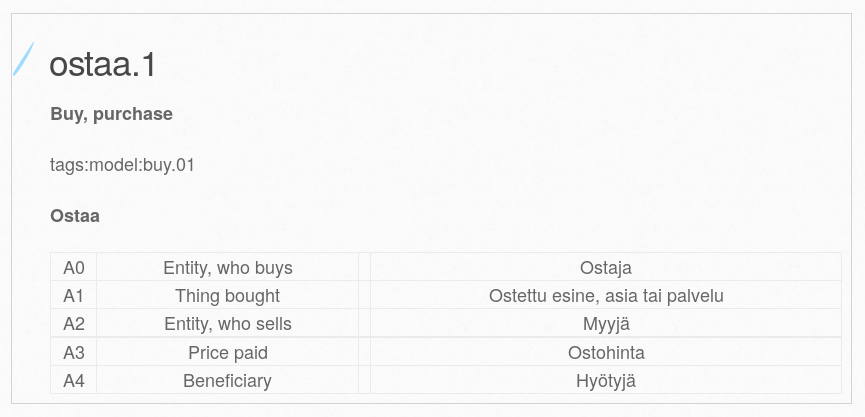
\includegraphics[width=0.8\textwidth]{graphics/finn-propbank.png}
\end{onlyenv}
\begin{onlyenv}<2>
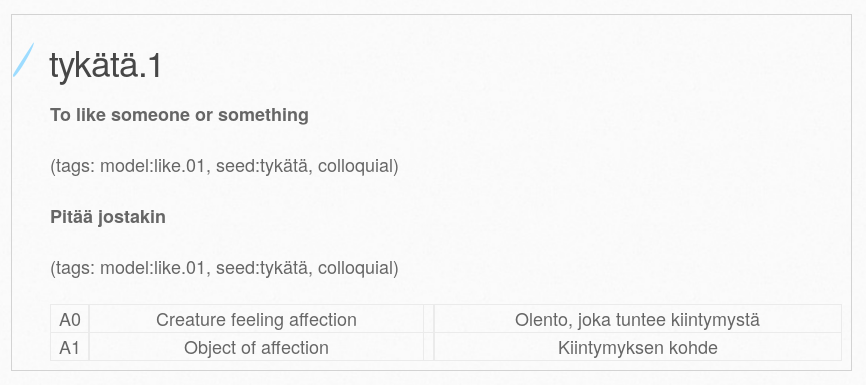
\includegraphics[width=0.8\textwidth]{graphics/finn-propbank2.png}
\end{onlyenv}
\end{center}

\begin{itemize}
  \item Finnish PropBank is freely available
  \item \url{https://github.com/TurkuNLP/Finnish_PropBank} (data branch)
\end{itemize}
  
\end{frame}

\begin{frame}{PropBank/5}

PropBank-style annotation allows us to see commonalities:

\scalebox{0.8}{
    \begin{dependency}[edge style={black,very thick}]
      \begin{deptext}[column sep=1mm,column 1/.style={anchor=base west}]
                        Maša \& myi \& kirjan \& Dašalle \& metrossa \\
                    \emph{ Маша }\&\emph{ продала }\&\emph{ книгу }\&\emph{ Даше }\&\emph{ в метро} \\
        \end{deptext}
        \depedge{2}{1}{nsubj}
        \depedge{2}{3}{obj}
        \depedge{2}{4}{obl}
        \depedge{2}{5}{obl}
        \depedge[edge below=true,edge style={red,very thick}]{2}{1}{{\sc arg2}}
        \depedge[edge below=true,edge style={red,very thick}]{2}{3}{{\sc arg1}}
        \depedge[edge below=true,edge style={red,very thick}]{2}{4}{{\sc arg0}}
    \end{dependency}
}

\scalebox{0.8}{
    \begin{dependency}[edge style={black,very thick}]
      \begin{deptext}[column sep=1mm,column 1/.style={anchor=base west}]
                        Daša \& osti \& kirjan \& Mašalta \& metrossa \\
                    \emph{ Даша}\&\emph{ купила}\&\emph{ книгу }\&\emph{ у Маши }\&\emph{ в метро} \\
        \end{deptext}
        \depedge{2}{1}{nsubj}
        \depedge{2}{3}{obj}
        \depedge{2}{4}{obl}
        \depedge{2}{5}{obl}
        \depedge[edge below=true,edge style={red,very thick}]{2}{1}{{\sc arg0}}
        \depedge[edge below=true,edge style={red,very thick}]{2}{3}{{\sc arg1}}
        \depedge[edge below=true,edge style={red,very thick}]{2}{4}{{\sc arg2}}
    \end{dependency}
}

\end{frame}

\begin{frame}{PropBank/6}

Summary:

\begin{itemize}
  \item A propbank is a corpus annotated with predicate--argument structure
  \item Predicate--argument structure generalises over syntax
  \item There is a free PropBank for Finnish
\end{itemize}

But how about Russian?

\begin{itemize}
  \item There is a semantically-annotated corpus based on FrameNet
  \item It could be converted into a PropBank 
  \item For more info ask Olya Lyashevskaya
\end{itemize}

\end{frame}

\begin{frame}{FrameNet/1}

FrameNet is very popular:

\begin{itemize}
  \item Semantically-annotated database/electronic resource
\end{itemize}

It contains (for English):
\begin{itemize}
  \item 1,200 frames
  \item 13,000 lexical units (word--meaning correspondence)
  \item 202,000 example sentences
\end{itemize}


\end{frame}



\begin{frame}{FrameNet/2}

\textbf{Frames:}
\begin{itemize}
  \item Conceptual structure involving participants, events and background knowledge
  \item Extremely specific, e.g. 
  \begin{itemize}
    \item \texttt{Commerce\_goods-transfer}
    \item \texttt{Being\_born}
    \item \texttt{Criminal\_process}
  \end{itemize}
\end{itemize}

\textbf{Frame elements:}
\begin{itemize}
  \item \textbf{Core:} essential to the meaning of the Frame
  \begin{itemize}
    \item \texttt{Seller}, \texttt{Buyer}, \texttt{Goods} 
  \end{itemize}
  
  \item \textbf{Non-core:} descriptive, e.g. time, place, manner 
  \begin{itemize}
     \item \texttt{Place}, \texttt{Purpose} 
  \end{itemize}
\end{itemize}

\end{frame}


\begin{frame}{vs. PropBank}

\textbf{PropBank:}

\begin{center}
\scalebox{0.8}{
    \begin{dependency}[edge style={black,very thick}]
      \begin{deptext}[column sep=1mm,column 1/.style={anchor=base west}]
                    \emph{ Маша }\&\emph{ продала }\&\emph{ книгу }\&\emph{ Даше }\&\emph{ в метро} \\
        \end{deptext}
        \depedge{2}{1}{nsubj}
        \depedge{2}{3}{obj}
        \depedge{2}{4}{obl}
        \depedge{2}{5}{obl}
        \depedge[edge below=true,edge style={red,very thick}]{2}{1}{{\sc arg2}}
        \depedge[edge below=true,edge style={red,very thick}]{2}{3}{{\sc arg1}}
        \depedge[edge below=true,edge style={red,very thick}]{2}{4}{{\sc arg0}}
    \end{dependency}
}
\end{center}

\textbf{FrameNet:}
\begin{center}
\begin{tabular}{ccccc}
\emph{ Маша }&\emph{ продала }&\emph{ книгу }&\emph{ Даше }&\emph{ в метро} \\
\texttt{Seller} &      ~    & \texttt{Goods}  & \texttt{Buyer} & \\
~              & продать.1 & ~                 & ~  & ~ \\
~              &     \texttt{Commerce\_goods-transfer}    & ~ & ~ & \\
\end{tabular}
\end{center}

\end{frame}


\begin{frame}[standout]
 Semantic role labelling
\end{frame}

\begin{frame}{Semantic role labelling}

A generic algorithm:
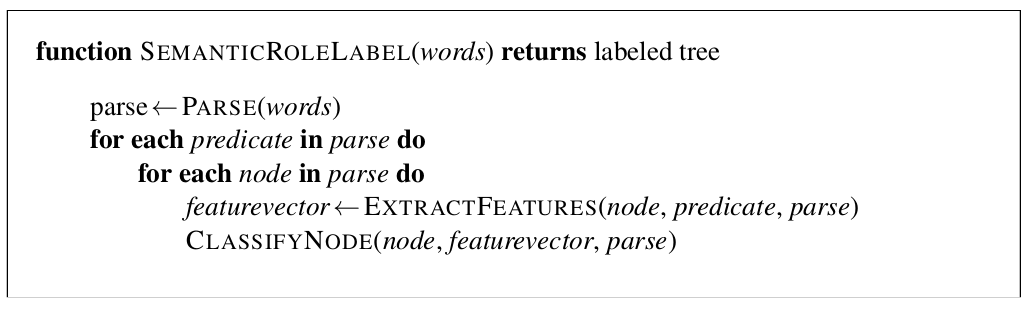
\includegraphics[width=\textwidth]{graphics/srl-parsing-algo.png}

How do we decide what is a predicate ?
\begin{itemize}
  \item \textbf{PropBank}: Use the verbs 
  \item \textbf{FrameNet}: Use what was labelled as such in the training data
\end{itemize}

\end{frame}

\begin{frame}{Features}

\begin{center}
\scalebox{0.7}{
    \begin{dependency}[edge style={black,very thick}]
      \begin{deptext}[column sep=1mm,column 1/.style={anchor=base west}]
            Rippeitä \& syötiin \& seuraavinakin \& päivinä \& , \& mutta \& se \& riitti \& minulle \\
            \emph{Leftovers} \& \emph{we ate} \& \emph{also following} \& \emph{days} \& \& \emph{but} \& \emph{that} \& \emph{sufficed} \& \emph{for me} \\
            \texttt{NOUN} \& \texttt{VERB} \& \texttt{ADJ} \& \texttt{NOUN} \& \& \texttt{CCONJ} \& \texttt{PRON} \& \texttt{VERB} \& \texttt{PRON} \\
              ~      \& {\sc syöda.1}         \& ~                      \& ~            \&  \&         \&             \& {\sc riittää.1} \&  \\
        \end{deptext}
        \depedge{2}{1}{obj}
        \depedge{2}{4}{obl}
        \depedge{4}{3}{amod}
        \depedge{8}{6}{cc}
        \depedge{8}{7}{nsubj}
        \depedge[edge unit distance=1.8ex]{2}{8}{conj}
        \depedge{8}{9}{obl}
        \depedge[edge below=true,edge style={red,very thick}]{2}{1}{{\sc Arg1}}
        \depedge[edge below=true,edge style={red,very thick}]{2}{4}{{\sc ArgM\_tmp}}
        \depedge[edge below=true,edge style={red,very thick}]{8}{7}{{\sc Arg1}}
        \depedge[edge below=true,edge style={red,very thick}]{8}{9}{{\sc Arg2}}
    \end{dependency}
}
\end{center}

\begin{onlyenv}<2>
\begin{tabular}{ll}
\hline
Headword of constituent & Rippeitä \\
Headword POS & NOUN \\
Headword Morph. features & Case=Par \\
Voice of clause & Active \\
Linear position (wrt. predicate) & before \\
Path features & ... \\
First and last words in constituent & ... \\
\hline
\end{tabular}
\end{onlyenv}


\end{frame}


\begin{frame}{One step or three step}

\textbf{One step}:
\begin{itemize}
  \item Classify argument type
\end{itemize}


\textbf{Three step}:
\begin{itemize}
  \item Prune unlikely nodes
  \item Identify if a node is an argument or not
  \item Classify argument type
\end{itemize}

Why add pruning and identification steps?

\end{frame}

\begin{frame}{Why add pruning and identification steps?}

\begin{itemize}
\item Algorithm is looking at one predicate at a time
\item Very few of the nodes in the tree could possible be arguments 
of that one predicate
\item Imbalance between: 
\begin{itemize}
\item (+) positive samples (constituents/nodes that are arguments of predicate)
\item (-) negative samples (constituents/nodes that are not arguments of predicate)
\end{itemize}
\item Imbalanced data can be hard for many classifiers
\item So we prune the very unlikely constituents first, and then use a classifier to get rid of the rest.
\end{itemize}

\end{frame}

\begin{frame}{Joint inference/1}

\begin{center}
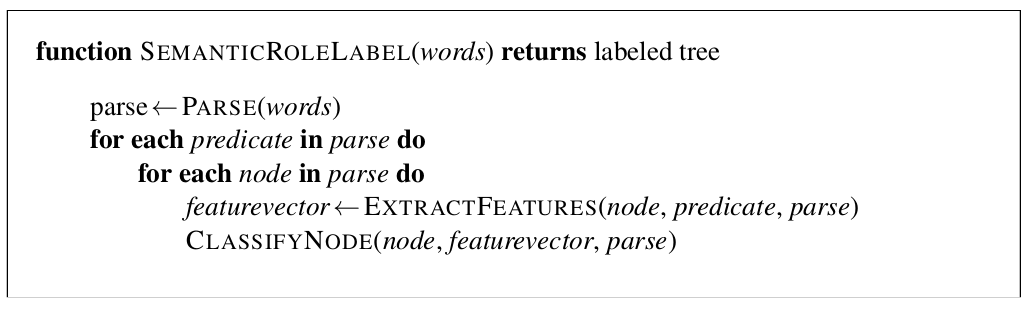
\includegraphics[width=0.8\textwidth]{graphics/srl-parsing-algo.png}
\end{center}

\begin{itemize}
\item The algorithm so far classifies everything  locally  -- each decision  about a constituent is made independently of all others
\item But: Lots of  global or joint interactions between arguments and constraints
\begin{itemize}
  \item e.g. PropBank does    not    allow    multiple    identical   arguments, so
  \item Labelling one constituent as Arg0 should increase the probability of another being Arg1
\end{itemize}
\end{itemize}

\end{frame}

\begin{frame}{Joint inference/2}

\textbf{Reranking}:
\begin{itemize}
\item The first stage SRL system produces multiple possible labels for each constituent
\begin{itemize}
 \item The second stage classifier the best  global label for  all constituents
 \item Often a classifier that takes all the inputs along with other features (sequences of labels)
\end{itemize}
\end{itemize}

\end{frame}

\begin{frame}{Summary}

\textbf{Semantic Role Labelling}:
\begin{itemize}
\item A level of shallow semantics for representing \textbf{events} and their \textbf{participants}
\item Intermediate between parses and full semantics
\item Two common architectures, for various languages
\begin{itemize}
\item FrameNet: frame-specific roles
\item PropBank: Proto-roles
\end{itemize}
\item Current systems extract by 
\begin{itemize}
\item parsing sentence
\item Finding predicates in the sentence
\item For each one, classify each parse tree constituent
\end{itemize}
\end{itemize}
\end{frame}

\begin{frame}[standout]

Practical

\end{frame}

\begin{frame}{Practical}
  
\textbf{Option 1:}
\begin{itemize}
  \item Download Finnish PropBank
  \begin{itemize}
     \item \url{https://github.com/TurkuNLP/Finnish_PropBank} 
     \item \url{https://github.com/TurkuNLP/Finnish_PropBank/tree/data} 
     \item \url{https://github.com/TurkuNLP/Finnish_PropBank/tree/data/gen_lemmas}
  \end{itemize}
  \item Write a semantic role labeller
  \item Train on {\tt train}, find good feature combination on {\tt dev} and test on {\tt test}.
\end{itemize}

\textbf{Option 2:}
\begin{itemize}
  \item Olya Lyaševskaya has given me a file with semantically annotated sentences for Russian
  \item Combination of TSV + XML
  \item Produce something approximating the PropBank style annotation.
\end{itemize} 

\end{frame}


\begin{frame}{Data format}
\emph{ Uusi elämä myös tuoksuu uudelta! :)} \\
`New life also smells fresh! :)'

\textbf{.conllu file}:

\scalebox{0.7}{
\begin{tabular}{llllllllll}
\textbf{ID} & \textbf{TOKEN} & \textbf{LEM}  & \textbf{POS} &  & \textbf{FEATS} & \textbf{HEAD} & \textbf{DEPREL} & \textbf{DEPRELS}& \textbf{MISC} \\
1           & Uusi           & \_ & \_ & \_ & \_ & 2             & amod            &  \_             & \_ \\
2           & elämä           & \_ & \_ & \_ & \_ & 4             & nsubj            &  4:PBArg\_1             & \_ \\
3           & myös           & \_ & \_ & \_ & \_ & 4             & advmod            & 4:PBArgM\_dis             & \_ \\
4           & tuoksuu           & \_ & \_ & \_ & \_ & 0             & root            &  \_             & PBSENSE=tuoksua.1\\
5           & uudelta           & \_ & \_ & \_ & \_ & 4             & xcomp            &  4:PBArg\_2             & \_ \\
6           & !           & \_ & \_ & \_ & \_ & 4             & punct            &  \_             & \_ \\
7           & :)           & \_ & \_ & \_ & \_ & 4             & discourse            &  \_             & \_ \\
\end{tabular}
}
~\\
~\\
\textbf{.tsv file}:
\begin{alltt}
\textbf{base|number|argnum|definition|note|definition\_fin|note\_fin} \\
tuoksua|1|1|Stinky thing|NULL|Tuoksuva asia|NULL \\
tuoksua|1|2|Attribute of arg1|NULL|Mille tuoksuu|NULL
\end{alltt}


\end{frame}

% Uusi elämä myös tuoksuu uudelta! :)
% New life also smells fresh! :)

% Rippeitä syötiin seuraavinakin päivinä, mutta se riitti minulle.
% We ate leftovers the next days too, but that was good enough for me

\begin{frame}

Combination of TSV + XML

\begin{tiny}
\begin{alltt}
\# new FrameAnno<br />\\
\# FrameAnchor = беречься<br />\\
\# ConstrID = 11655<br />\\
\# ConstrName = 1.5\_Берегись, чтобы не упасть.<br />\\
\# ConstrPattern = Snom V чтобы + CL<br />\\
\# ExampleID = 43401<br />\\
\# SentType = sp<br />\\
\# SentXml =     <p class="verse"><se><w><ana lex="плакать" gr="V,2p,act,imper,ipf,norm,sg" sem="ca:noncaus t:physiol d:root" sem2="ca:noncaus d:root"/>Плачь</w>, <w><ana lex="но" gr="CONJ,norm"/>но</w> <w><ana lex="беречься" gr="V,2p,act,imper,ipf,norm,sg" sem="ca:noncaus" sem2="ca:noncaus"/>берегись</w>, <w><ana lex="чтобы" gr="CONJ,norm"/>чтобы</w> <w><ana lex="хоть" gr="PART,norm"/>хоть</w> <w><ana lex="один" gr="APRO,f,nom,norm,sg" sem2="r:indet"/>одна</w> <w><ana lex="твой" gr="APRO,f,nom,norm,sg" sem="r:poss"/>твоя</w> ... \\
\# SentText =  <u>Плачь, но <b>берегись</b>, чтобы хоть одна твоя слеза скатилась по острию пера и примешалась к чернилам. </u>Ренар <br />\\
\# FEtable:FE\_ID	"Word"	Role	FE\_Status	SyntRank	Morph	LexClass	"Group"<br />\\
21184	""	агенс	Core	Не выражен			""<br />\\
21185	"берегись"	-	Core	Предикат	беречься	-	"-"<br />\\
21186	"что / скатилась"	потенциальная угроза	Core	Клауза	чтобы + CL	-	"чтобы хоть одна твоя слеза скатилась по острию пера и примешалась к чернилам"<br /><br /><br />\\
\end{alltt}
\end{tiny}


% Ženya: ``How was it born like that?'' 

\end{frame}


\end{document}

%  Tensions have not eased between the Catalan and Spanish governments following the vote.
%  Following the vote tensions in 
